\documentclass[11pt]{article}
\usepackage[pdftex]{graphicx}
\usepackage{url}

\setlength{\textwidth}{6.5in}
\setlength{\textheight}{9.25in}

\setlength{\voffset}{-0.0in}
\hoffset=-50pt
\topmargin=0pt
\headheight=0pt
\headsep=0pt
\evensidemargin=72pt % 1in+7pt

\setlength{\parskip}{0.5ex}
\setlength{\parindent}{1em}
\setlength{\floatsep}{1pt}
\setlength{\textfloatsep}{2pt}
\setlength{\intextsep}{2pt}

\begin{document}

\title{Map{R}educe in {MPI} for Large-scale Graph Algorithms}

\author{
Steven J.~Plimpton and Karen D.~Devine \\
Sandia National Laboratories \\
Albuquerque, NM \\
sjplimp@sandia.gov
}

\date{}

\maketitle

\centerline{Keywords: MapReduce, message-passing, MPI, graph
algorithms, R-MAT matrices}

\vspace*{0.4in}

\begin{abstract}

We describe a parallel library written with message-passing (MPI)
calls that allows algorithms to be expressed in the MapReduce
paradigm.  This means the calling program does not need to include
explicit parallel code, but instead provides ``map'' and ``reduce''
functions that operate independently on elements of a data set
distributed across processors.  The library performs needed data
movement between processors.  We describe how typical MapReduce
functionality can be implemented in an MPI context, and also in an
out-of-core manner for data sets that do not fit within the aggregate
memory of a parallel machine.  Our motivation for creating this
library was to enable graph algorithms to be written as MapReduce
operations, allowing processing of terabyte-scale data sets on 
traditional MPI-based clusters.  We
outline MapReduce versions of several such algorithms: vertex ranking
via PageRank, triangle finding, connected component identification,
Luby's algorithm for maximally independent sets, and single-source
shortest-path calculation.  To test the algorithms on arbitrarily
large artificial graphs we generate randomized R-MAT matrices in
parallel; a MapReduce version of this operation is also described.
Performance and scalability results for the various algorithms are
presented for varying size graphs on a distributed-memory cluster.
For some cases, we compare the results with non-MapReduce algorithms,
different machines, and different MapReduce software, namely Hadoop.
Our open-source library is written in C++, is callable from C++, C,
Fortran, or scripting languages such as Python, and can run on any
parallel platform that supports MPI.

\end{abstract}

\vspace*{0.4in}

\centerline{29 Nov 2010 version}
\centerline{To appear in special issue of Parallel Computing.}

\pagebreak

\section{Introduction}
\label{sec:intro}

MapReduce is the programming paradigm popularized by Google
researchers Dean and Ghemawat \cite{Dean}.  Their motivation was to
enable rapid development and deployment of analysis programs to
operate on massive data sets residing on Google's large distributed
clusters.  They introduced a novel way of thinking about certain kinds
of large-scale computations as a "map" operation followed by a
"reduce" operation.  The power of the paradigm is that when cast in
this way, a nominally serial algorithm now becomes two highly parallel
operations working on data local to each processor, sandwiched around
an intermediate data-shuffling operation that requires inter-processor
communication.  The user need only write serial code for the
application-specific map and reduce functions; the parallel data
shuffle can be encapsulated in a library since its operation is
independent of the application.

The Google implementation of MapReduce is a C++ library with
communication between networked machines via remote procedure calls.
It allows for fault tolerance when large numbers of machines are used,
and can use disks as out-of-core memory to process petabyte-scale data
sets.  Tens of thousands of MapReduce programs have since been written
by Google researchers and are a significant part of the daily compute
tasks run by the company \cite{Dean2}.

Similarly, the open-source Hadoop implementation of MapReduce
\cite{Hadoop}, has become widely popular in the past few years for
parallel analysis of large-scale data sets at Yahoo and other
data-centric companies, as well as in university and laboratory
research groups, due to its free availability.  MapReduce programs in
Hadoop are typically written in Java, though it also supports use of
stand-alone map and reduce kernels, which can be written as shell
scripts or in other languages.

More recently, MapReduce formulations of traditional number-crunching
kinds of scientific computational tasks have been described, such as
post-processing analysis of simulation data \cite{Tu}, graph
algorithmics \cite{Cohen}, and linear algebra operations \cite{Fox}.
The paper by Tu et al \cite{Tu} was particularly insightful to us,
because it described how MapReduce could be implemented on top of the
ubiquitous distributed-memory message-passing interface (MPI), and how
the intermediate data-shuffle operation is conceptually identical to
the familiar $MPI_Alltoall$ operation.  Their implementation of
MapReduce was within a Python wrapper to simplify the writing of user
programs.  The paper motivated us to develop our own C++ library built
on top of MPI for use in graph analytics, which we initially released
as open-source software in mid-2009 \cite{MRMPI}.  We have since
worked to optimize several of the library's underlying algorithms and
to enable its operation in out-of-core mode on larger data sets.
These algorithmic improvements are described in this paper and are
part of the current downloadable version \cite{MRMPI}.

The MapReduce-MPI (MR-MPI) library described in this paper is a
simple, lightweight implementation of basic MapReduce functionality,
with the following features and limitations:

\begin{itemize}

\item {\it C++ library using MPI for inter-processor communication:}
The user writes a (typically) simple main program which runs on each
processor of a parallel machine, making calls to the MR-MPI library.
For map and reduce operations, the library calls back to user-provided
map() and reduce() functions.  The use of C++ allows precise control
over the memory and format of data allocated by each processor during
a MapReduce.  Library calls for performing a map, reduce, or data
shuffle, are synncrhonous, meaning all the processors participate and
finish the operation before proceeding.  Similarly, the use of MPI
within the library is the traditional mode of $MPI_Send()$ and
$MPI_Recv$ calls between processor pairs using large aggregated
messages to improve bandwidth performance and reduce latency costs.  A
recent paper by \cite{Dongarra} also outlines the MapReduce formalism
from an MPI perspective, though they advocate a more asyncrhonous
approach, using one-way communication of small messages.

\item {Small, portable:} The entire MR-MPI library is a few thousand
lines of standard C++ code.  For parallel operation, the program is
linked with MPI, a standard message passing library available on all
distributed memory machines.  For serial operation, a dummy MPI
library (provided) can be substituted.

\item {\it In-core or out-of-core operation:} Each MapReduce object a
processor defines, allocates per-processor "pages" of memory, where
the page size is determined by the user.  Typical MapReduce operations
can be performed using a few such pages.  If the data set fits in a
single page (per processor), then the library performs its operations
in-core.  If the data set exceeds the page size, then processors each
write to temporary disk files (to local disk or a parallel file
system) as needed and subsequently read from them.  This allows
processing of data sets larger than the aggregate memory of all the
processors, i.e. up to the available aggregate disk space.

\item {\it Flexible programmability:} An advantage of writing a
MapReduce program on top of MPI, is that the user program can invoke
MPI calls directly, if desired.  For example, one-line calls to
$MPI_Allreduce$ are often useful in determining the status of an
iterative graph algorithm, as described in Section \ref{sec:graph}.
The library interface also provides a user data pointer as an argument
passed back to all callback functions, so it is easy for the user
program to store ``state'' on each processor, accessible during the
map and reduce operaions.  For example, various flags can be stored
that alter the operation of a map or reduce function, as can richer
data structures, that accumulate the results.

\item {\it C++, C, and Python interfaces:} A C++ interface to the
MR-MPI library means a user program instantiates and then invokes
methods in one or more MapReduce objects.  A C interface means the
library can also be called from C or other hi-level languages such as
Fortran.  A C interface also means the library can be easily wrapped
by Python via the Python ``ctypes'' module.  The library can then be
called from a Python script, allowing the user to write map() and
reduce() callback functions in Python.  If a machine supports running
Python in parallel, a parallel MapReduce can also be run in this mode.

\item {No fault tolerance:} Current MPI implementations do not enable
easy detection of a dead processor, or retrieval of the data it was
working on.  So like most MPI programs, a parallel program calling the
MR-MPI library will hang or crash if a processor goes away.  Unlike
Hadoop, and its HDFS file system which provides for data redundancy,
the MR-MPI library simply reads and writes simple, flat files.  It can
use local per-processor disks, or a parallel file system, if
available, but these typically provide no data redundancy.

\end{itemize}

The remainder of the paper is organized as follows.  The next two
sections \ref{sec:mr} and \ref{sec:outcore} describe how in-core and
out-of-core MapReduce primitives are formulated as MPI-based
operations in the MR-MPI library.  Section \ref{sec:graph} briefly
describes the formulation of several common graph algorithms as
MapReduce operations.  Section \ref{sec:results} gives performance
results for these algorithms running on a parallel cluster for graphs
ranging in size from 1 million to 1 trillion vertices or edges.  In
this section, we highlight the performance and complexity trade-offs
of a MapReduce approach versus other more special-purpose algorithms.
The latter generally perform better but are harder to implement
efficiently on distributed memory machines, due to the required
explicit management of parallelism, particularly for large out-of-core
data sets.  Section \ref{sec:lessons} summarizes some lessons learned
from the implementation and use of our library.

\section{MapReduce in MPI}
\label{sec:mr}

The basic datums stored and operated on by any MapReduce framework are
key/value (KV) pairs.  In the MR-MPI library, individual keys or
values can be of any data type or length, or combinations of multiple
types (one integer, a string of characters, two integers and a double,
etc); they are simply treated as byte strings by the library.  A KV
pair always has a key; its value may be NULL.  KV pairs are stored
within a MapReduce (MR) object.  A user program may create one or more
MR objects to implement an algorithm.  Various MapReduce operations
(map, reduce, etc) are invoked on an object and its KV pairs; KV pairs
can also be passed between and combined across objects.

A related data type in the MR-MPI library is the key/multivalue (KMV)
pair, where all values associated with the same key are collected and
stored contiguously as a multivalue, which is just a longer byte
string with an associated vector of lengths, one integer length per
value.  In this section, we assume the KV and KMV datums operated on
by each processor fit in local memory.

A typical MR-MPI program makes at least three calls to the MR-MPI
library, to perform {\it map()}, {\it collate()}, and {\it reduce()}
operations on a MR object it creates.  In a {\it map()}, zero or more
key/value pairs are generated by each processor.  Often this is done
using data read from files, but a {\it map()} may generate data itself
or process existing KV pairs to create new ones.  The KV pairs
produced are stored locally by each processor; a {\it map()} thus
requires no inter-processor communication.  Users call the library
with a count of tasks to perform and a pointer to a user function; the
MR-MPI {\it map()} operation invokes the user function multiple times
as a callback.  Depending on which variant of {\it map()} is called,
the user function may be passed a file name, a chunk of bytes from a
large file, a task ID, or a KV pair.  Options for assigning map tasks
to processors are specified by the user and include assigning
consecutive chunks of tasks to processors, striding the tasks across
processors, or using a master-slave model that is useful when tasks
have widely varying workloads.

The {\it collate()} operation (or data shuffle in Hadoop) identifies
unique keys and collects all the values associated with those keys to
create KMV pairs.  This is done in two stages, the first of which
requires communication, since KV pairs with the same key may be owned
by any processor.  Each processor hashes each of its keys to determine
which processor will ``own'' it.  The $k$-byte length key is hashed
into a 32-bit value whose remainder modulo $P$ processors is the
owning processor rank.  Alternatively, the user can provide a hash
function that converts the key into a processor rank.  Each processor
then sends each of its KV pairs to the owning processor.

After receiving new KV pairs, the second stage is an on-processor
computation, requiring no further communication.  Each processor
reorganizes its KV pairs into KMV pairs, one for each unique key it
owns.  This is done using a hash table, rather than a sort.  A sort
scales as $N\log_2(N)$, i.e. it requires $\log_2(N)$ passes through
the $N$ KV pairs.  With hashing, the list of KMV pairs can be created
in two passes.  The first pass populates the hash table with needed
count and length information; the second pass copies the key and value
datums into the appropriate location in a new KMV data structure.
Since the cost to lookup a key in a well-formed hash table is a
constant-time $O(1)$ operation, the cost of the data reorganization is
also $O(N)$.  This methodology has the added benefit that the number
of values in each KMV pair is known and can be passed to the user
function during a reduce.  For some reduce operations, this count is
all the information a reduce requires; the values need not be looped
over.  The count is not available in Hadoop-style data shuffles, which
sort the values; counting the values associated with the same key
requires iterating over the values.

Note that the first portion of the {\it collate()} operation involves
all-to-all communication since each processor exchanges KV pairs with
every other processor.  The communication can either be done via a
MPI\_Alltoall() library call, or by a custom routine that aggregates
datums into large messages and invokes point-to-point MPI\_Send() and
MPI\_IRecv() calls.

The {\it reduce()} operation processes KMV pairs and can produce new
KV pairs for continued computation.  Each processor operates only on
the KMV pairs it owns; no communication is required.  As with the {\it
map()}, users call the library with a pointer to a user function.  The
MR-MPI {\it reduce()} operation invokes the user function, once for
each KMV pair.

Several related MapReduce operations are provided by the library.  For
example, the {\it collate()} function described above calls two other
functions: {\it aggregate()}, which performs the all-to-all
communication, and {\it convert()}, which reorganizes a set of KV
pairs into KMV pairs.  Both functions can be called directly.  The
{\it compress()} function allows on-processor operations to be
performed; it is equivalent to a {\it convert()} with on-processor KVs
as input, followed by a {\it reduce()}.  The {\it clone()} function
turns a list of KV pairs into KMV pairs, with one value per key.  The
{\it collapse()} function turns $N$ KV pairs into one KMV pair, with
the keys and values of the KV pairs becoming $2N$ values of a single
multivalue assigned to a new key.  The {\it gather()} function
collects KV pairs from all processors to a subset of processors; it is
useful for doing output from one or a few processors.  Library calls
for sorting datums by key or value or for sorting the values within
each multivalue are also provided.  These routines invoke the
C-library {\it quicksort()} function to compute the sorted ordering of
the KV pairs (or values within a multivalue), using a user-provided
comparison function.  The KV pairs (or values in a multivalue) are
then copied into a new data structure in sorted order.

The interface to various low-level operations is provided so that a
user's program can string them together in various ways to construct
useful MapReduce algorithms.  For example, output from a {\it
reduce()} can serve as input to a subsequent {\it map()} or {\it
collate()}.  Likewise, data can be partitioned across multiple
MapReduce (MR) objects, each with its own set of KV pairs.  For
example, as will be illustrated in Section~\ref{sec:graph}, one MR
object can store the edges of a graph, and another its vertices.  KV
pairs from multiple MR objects can be combined to perform new
sequences of {\it map()}, {\it collate()}, and {\it reduce()}
operations.

The above discussion assumed that the KV or KMV pairs stored by a
processor fit in its physical memory.  In this case, the MR-MPI
library performs only ``in-core'' processing and no disk files are
written or read by any of the processors, aside from initial input
data (if it exists) or final output data (if it is generated).  Note
that the aggregate physical memory of large parallel machines can be
multiple terabytes, which allows for large data sets to be processed
in-core, assuming the KV and KMV pairs remain evenly distributed
across processors throughout the sequence of MapReduce operations.
The use of hashing to assign keys to processors typically provides for
such load-balancing.  In the next section, we discuss what happens
when data sets do not fit in available memory.

\section{Out-of-core Issues}
\label{sec:outcore}

  what part needs to be out-of-core in MPI context
  each proc does it's own disk IO
  basic idea: modified data structures for KV and KMV
  map() operation
  aggreate() operation
  convert() operation
  reduce() operation

If the set of key/value or key/multivalue pairs generated or owned by
a processor exceeds the {\it memsize} of its allocated memory, then
MR-MPI switches to ``out-of-core'' processing.  Each processor uses
temporary files to store data that does not fit in its memory.
Depending on the parallel machine's hardware configuration, these
files can reside on disks local to each processor, on the front end
(typically a NSF-mounted file system for a parallel machine), or on a
parallel file system/disk array.  The files are read/written as large
contiguous ``pages'', which are 1/4 the size of the {\it memsize}
setting discussed in the previous section.

We now explain how the MapReduce primitives described above operate in
out-of-core mode.  The {\it map()} and {\it reduce()} operations are
relatively simple.  As a {\it map()} generates key/value pairs, it
fills up a page, one key/value pair at a time.  When the page is full,
it is written to disk.  If the source of data for the {\it map()}
operation is an existing set of key/value pairs, then those datums are
read in, one page at a time, and each key/value pair is given to the
user map() function.  Similarly, a {\it reduce()} reads one page of
key/multivalue pairs from disk, passes them one at a time to the user
reduce() function, which typically generates new key/value pairs.  The
generated pairs fill up a new page, which is written to disk when
full, just as with the {\it map()} operation.  Thus for both a {\it
map()} and {\it reduce()}, out-of-core disk files are read and written
sequentially, one page at a time.

A special case is when a single key/multivalue pair is larger than a
single page.  This can happen, for example, in a connected component
finding algorithm if the graph collapses into one or a few giant
components.  In this case, the entire set of values (graph vertices
and edges) associated with the unique key (the component ID), may not
fit in one page of memory.  The individual values in the multivalue
will then be spread across as many pages as needed.  The user reduce()
function is passed a flag indicating it is receiving only a portion of
the values.  Once it has processed them, it can request a new set of
values (from a new page) from the MR-MPI library.

Performing a {\it collate()} operation out-of-core is more complex.
Recall that a collate() operation occurs in two stages.  First, keys
are hashed to ``owning'' processors and the key/value data is
communicated in an all-to-all fashion.  This is done one page of
key/value data at a time.  Each processor reads in a page of key/value
data, the communication pattern is determined (who needs what datums),
and the communication is performed.  So long as each processor
receives no more than 2x its share of the datums (one page), it has
room to receive it within the {\it memsize} restriction.  If the
key/value data is load-imbalanced so that this limit is exceeded, then
the all-to-all communication can be performed in multiple passes.

When the first stage is done, each processor now has an out-of-core
set of key/value datums that need to be reorganized into an
out-of-core set of key/multivalue pairs.  In principle, to create one
page of key/multivalue data, the entire set of key/value pairs needs
to be scanned to find all keys which contribute values to that page.
Reading all the key/value pages from disk for each page of
key/multivalue output could be prohibitively expensive.  A related
issue is that a hash table is needed to match new keys with previously
encountered keys.  But there is no guarantee that the hash table
itself will fit within the memory specified by the user via the {\it
memsize} parameter.  Our solution to these issues is to partition the
{\it memsize} memory into 3 pieces: 2 pieces each of size {\it
memsize}/4 for reading/writing pages of key/value and key/multivalue
pairs, and the remaining {\it memsize}/2 piece for a hash table.  We
can then scan the key/value pairs at most four times to produce all
the pages of key/multivalue output, as diagrammed in Figure
\ref{f:collate}.

\begin{figure}
\includegraphics[width=\textwidth,angle=-90]{fig_collate.pdf}
\caption{Four-pass algorithm for converting key/value data to
key/multivalue data.  The vertical lines represent out-of-core data
sets.  KV is key/value pairs; HT is an in-memory hash table; KMV is
key/multivalue pairs.}
\label{f:collate}
\end{figure}

\begin{itemize}

\item (Pass 1) The key/values are read and split into two files.  The
first file contains all the key/values pairs whose keys fit into the
finite-size hash table.  The second contains those which do not.

\item (Pass 2) The size of the first file (generally smaller) can be
used to estimate how many chunks the second file (generally larger)
needs to be partitioned into so that each chunk contains a set of
unique keys than can fit into the hash table.  This estimate is made
conservatively so that additional passes through the data are almost
never required.  The second pass thus reads the larger file and writes
out smaller files, similar in size to the first file created by the
first pass.

\item (Pass 3) The unique keys in each small file of key/value pairs
can now be hashed, but the file may contain more value data than will
fit in one key/multivalue page.  As each small file is read, and its
keys hashed, the accumulating hash table statistics can be used to
determine which key/values correspond to single pages of
key/multivalue output.  The key/values can thus be split into even
smaller files, one for each key/multivalue page.

\item (Pass 4) Each smaller file of key/value pairs is read, its keys
hashed, and the key/value data reorganized into sequential
key/multivalue pairs which fill a key/multivalue page, which is then
written out to disk.

\end{itemize}

Note that depending on the data set size and its key distribution all
four passes through the data may not be necessary, but the upper limit
is four, assuming the chunk-size estimations are accurate.  By
comparison, a merge sort of key/value pairs would require $log_2(N)$
passes (read/write) through the out-of-core data set, where $N$ is its
number of pages.  The MR-MPI {\it collate()} operation does not
actually sort the key/multivalue pairs by key; the final ordering is
indeterminate as it is created by the hash function.

The other MR-MPI library calls ({\it compress()}, {\it gather()},
sorting by key or value, etc) can also operate in out-of-core mode,
typically with one pass through the key/value or key/multivalue data.
Sorting is an exception, as an out-of-core merge sort requires
$log_2(N)$ passes, as just mentioned, where $N$ is the number of
pages.

\section{Graph Algorithms in MapReduce}
\label{sec:graph}

We begin with a MapReduce procedure for creating large, sparse,
randomized graphs, since they are the input for the algorithms
discussed below.  R-MAT graphs ~\cite{RMAT} are recursively generated
graphs with power-law degree distributions.  They are commonly used to
represent web and social networks.  The user specifices six parameters
that define the graph: the number of vertices $N$ and edges $M$, and
four parameters $a$, $b$, $c$, $d$ that sum to 1.0 and are discussed
below.  The algorithm in Figure~\ref{fig:rmat} generates $M$ unique
non-zero entries in a sparse $N \times N$ matrix $A$, where each entry
$A_{ij}$ represents an edge between graph vertices $(V_i,V_j)$.

\begin{figure}[htb]
 \begin{center}\fbox{\begin{minipage}{\textwidth} \begin{tabbing}
  xxxx\=xxxxxxxxxxxx\=xxxxxxxxxxxxxxxxxxxxxxxxxxxxxxxxxx\= \kill

$M_{\rm remain} = M$ \\
while $M_{\rm remain} > 0$: \\
\> Map: \> Generate $M_{\rm remain}/P$ random edges on each processor \\
           \> \> output Key = $(i,j)$, Value = NULL \\
\> Collate \\
\> Reduce: \> Remove duplicate edges \\
           \> \> input Key = $(i,j)$, MultiValue = one or more NULLs \\
           \> \> output Key = $(i,j)$, Value = NULL \\
\> $M_{\rm remain} = M - N_{kv}$

  \end{tabbing}
 \end{minipage}}\end{center}

 \caption{MapReduce algorithm for R-MAT graph generation.}

 \label{fig:rmat}
\end{figure}

In the {\it map()} operation, each of $P$ processors generates a $1/P$
fraction of the desired edges.  A single random edge ($i,j$) is computed
recursively as follows.  Pick a random quadrant of the $A$ matrix with
relative probabilities $a$, $b$, $c$, and $d$.  Treat the chosen
quadrant as a sub-matrix and select a random quadrant within it, in
the same manner.  Repeat this process $n$ times where $N = 2^n$.  At
the end of the recursion, the final ``quadrant'' is non-zero matrix
element $A_{ij}$.

The {\it map()} will often generate some small number of duplicate edges.
The {\it collate()} and {\it reduce()} operations remove the duplicates.  The
entire map-collate-reduce sequence is repeated until the number of
resulting key/value pairs $N_{kv} = M$.  For reasonably sparse graphs
this typically takes only a few iterations.

Note that the degree distribution of vertices in the graph depends on
the choice of parameters $a$, $b$, $c$, $d$.  If one of the four
values is larger than the other three, a highly skewed distribution
results.  Variants of the above algorithm can be used when $N$ is not
a power-of-two, to generate graphs with weighted edges (assign a
numeric value to the $A_{ij}$ edge), graphs without self edges
(require $i \ne j$), or graphs with undirected edges (require $i < j$).
Or the general R-MAT matrix can be further processed by MapReduce
operations to meet these requirements.  For some algorithms below
(e.g., triangle finding and maximal independent set generation), we
post-process R-MAT matrices to create upper-triangular R-MAT
matrices representing undirected graphs.  For each edge $(i,j)$ 
with $i>j$, we add edge $(j,i)$, essentially symmetrizing the matrix; 
we then remove duplicate edges and self edges,
leaving only edges with $i<j$.

By using more than one MapReduce object, we can improve the performance
of the R-MAT generation algorithm, particularly when out-of-core operations
are needed.  In the enhanced algorithm
(Figure~\ref{fig:rmat2}), we emit newly created edges into MapReduce object
$E_{new}$ and {\it aggregate()} the edges to processors.  
We then add those edges
to the MapReduce object $E_{old}$, containing all previously generated
unique edges; the edges of $E_{old}$ are already aggregated to processors
using the same mapping as $E_{new}$.  We can then use the {\it compress()}
function to reduce duplicates locally on each processor.
Time reductions
in this algorithm result from the reduced number of KV pairs communicated in
{\it aggregate()},
compared to the collate operation in the original algorithm, 
particularly in later iterations of the generation where few
edges are created.

\begin{figure}[htb]
 \begin{center}\fbox{\begin{minipage}{\textwidth} \begin{tabbing}
  xxxx\=xxxxxxxxxxxx\=xxxxxxxxxxxxxxxxxxxxxxxxxxxxxxxxxx\= \kill

$M_{\rm remain} = M$ \\
while $M_{\rm remain} > 0$: \\
\> Map $E_{new}$: \> Generate $M_{\rm remain}/P$ random edges on each processor \\
           \> \> output Key = $(i,j)$, Value = NULL \\
\> Aggregate $E_{new}$. \\
\> Add $E_{new}$ to $E_{old}$. \\
\> Compress $E_{old}$: Remove duplicate edges \\
            \> \> input Key = $(i,j)$, MultiValue = one or more NULLs \\
            \> \> output Key = $(i,j)$, Value = NULL \\
\> $M_{\rm remain} = M - N_{kv}$

  \end{tabbing}
 \end{minipage}}\end{center}

 \caption{Enhanced MapReduce algorithm for R-MAT graph generation.}

 \label{fig:rmat2}
\end{figure}

\subsection{PageRank}

The PageRank algorithm assings a relative numeric rank to each
vertex in a graph.
It models the web as a directed graph $G(V,E)$, with each vertex $V_i
\in V$ representing a web page and each edge $(V_i, V_j) \in E$
representing a hyperlink from $V_i$ to $V_j$.  The probability of
moving from $V_i$ to another vertex $V_j$ is $\alpha/d_{out}(V_i) +
(1-\alpha)/|V|$, where $\alpha$ is a user-defined parameter (usually
0.8-0.9), $d_{out}(V_i)$ is the outdegree of vertex $V_i$, and $|V|$ is
the cardinality of $V$.  The first term represents the probability of
following a given link on page $V_i$; the second represents the
probability of moving to a random page.  For pages with no outlinks,
the first term is $\alpha/|V|$, indicating equal likelihood to move to
any other page.  Equivalently, the graph can be represented by a
matrix $A$~\cite{LangvilleMeyer05a}, with matrix entries $A_{ij} =
\alpha/d_{out}(V_i)$ if vertex $V_i$ links to $V_j$.  To maintain the 
sparsity of $A$, terms for random jumps and zero out-degree vertices are
not explicitly stored in $A$.  Rather, they are computed separately
as adjustments to the PageRank vector.  The kernel of the PageRank
algorithm, then, is a power-method iteration consisting of 
matrix-vector multiplication $A^T x=y$,
where $x$ is the PageRank vector from the previous iteration, and
a few dot product and norm computations.

The algorithm in Figure~\ref{fig:pr} performs these
iterations.  The nonzeros of matrix $A$ are initialized as described above;
the PageRank vector $x$ is initialized uniformly.  A MapReduce object $MT$
contains the indices of all-zero rows of $A$, corresponding to vertices
with no outlinks.  In step 1 of a PageRank interation, $MT$ is used 
in dot products to compute adjustments to the
PageRank vector to represent uniform probability of going from a leaf page
to any other page.  Adjustments for random jumps from any page are also
computed in this step.  Step 2, the matrix-vector product $A^T x$, is the most
expensive part of the computation, requiring two passes over the nonzero
structure of $A$.  In the first pass, {\it collate()} 
gathers all row entries $a_{ij}$ with their
associated $x_i$ entry, and {\it reduce()} computes $a_{ij} x_i$.  
In the second pass, 
{\it collate()} gathers, for each $j$, all contributions to the
column sum $\sum_i a_{ij} x_i$, which is computed by a second {\it reduce()}. 
Steps 3 and 4 adjust and scale the 
product vector; the work is proportional to $|V|$.  Step 6 computes the
residual to determine whether the PageRank vector has converged; work is
again proportional to $|V|$.  Throughout the algorithm, we exploit the
ability to call MPI\_Allreduce to compute global norms and residuals. 

\begin{figure}[htb]
 \begin{center}\fbox{\begin{minipage}{\textwidth} \begin{tabbing}
  xxxx\=xxxxx\=xxxxx\=xxxxx\=xxxxxxxxxxxxxxxxxxxxxxxxxxx\= \kill

%Input from R-MAT generator: \\
%\> MapReduce object $V$ containing all graph vertices:  Key=$V_i$, Value = NULL.  \\
%\> MapReduce object $E$ containing all graph edges: Key=$V_i$, Value = $V_j$. \\
%Initialize MapReduce object for matrix $A$  and \\
%MapReduce object $MT$ containing all vertices with no outlinks.\\
%\> Copy: $A = E$ \\
%\> Add: $V$ to $A$ \\
%\> Collate $A$: Vertex is Key \\
%\> Reduce $A$:  \\
%\> \> Input:  Key = $V_i$; MultiValue = NULL,$V_j$,$V_k$,... \\
%\> \> If (${nvalues} > 1$) \\
%\> \> \> Compute: $d_{out}(V_i) = {nvalues} - 1$. \\
%\> \> \> Output:  For each $V_j$ in MultiValue, Key = $V_i$; Value = ($V_j$, $\alpha/d_{out}(V_i)$). \\
%\> \> else \\
%\> \> \> Output to $MT$: Key = $V_i$; Value = 0. \\
%Initialize MapReduce object for pagerank vector $x$. \\
%\> Map:   \\
%\> \> Input:  Graph vertices $V$. \\
%\> \> Output:  For each vertex, Key = $V_i$; Value = $1/|V|$. \\
Input: \\
\> MapReduce object $A$ containing $|V| \times |V|$ matrix:  Key = $i$, Value = $[j, a_{ij}]$ \\
\> MapReduce object $MT$ containing indices of all-zero rows of $A$:  Key = $i$, Value = 0. \\
\> MapReduce object $x$ containing initial PageRank vector:  Key = $i$, Value = $1/|V|$. \\
While (${residual} > {tolerance}$) \\
\> 1. Compute contribution for random jumps and zero-outdegree vertices. \\
\> \> Add: $x$ to $MT$. \\
\> \> Collate $MT$:  Vertex is Key. \\
\> \> Reduce $MT$:   \\
\> \> \> Input:  Key = $i$; MultiValue = $x_i, 0$ if $i \in {MT}$; MultiValue = $x_i$ if $i \notin {MT}$. \\
\> \> \> Compute:  Local contributions $c_{local}$. \\
\> \> \> Output:  If ${nvalues} = 2$, Key = $i$; Value = 0. \\
\> \> MPI\_Allreduce $c_{local}$ with MPI\_SUM to compute global contribution $c_{global}$. \\
\> 2. Compute $y = A^T x$.  \\
\> \> Copy $x$ to $y$. \\
\> \> Add $A$ to $y$. \\
\> \> Collate $y$:  Key is row index of $A$. \\
\> \> Reduce $y$: \\
\> \> \>  Input: Key = $i$; Multivalue = $i, [j, a_{ij}]$ for nonzeros $a_{ij}$ in $A$ \\
\> \> \>  Output:  Key = $j$; Value = $a_{ij} y_i$. \\
\> \> Collate $y$:  Key is column index of $A$. \\
\> \> Reduce $y$:  \\
\> \> \> Input:  Key = $j$; Multivalue = $a_{ij} y_i$ for all non-zero entries $a_{ij}$ of column $j$ \\
\> \> \> Output:  Key = $j$; Value = $\sum_i a_{ij} y_i$. \\
\> 3. Add contribution $c_{global}$ to $y$; compute local max norm $n_{local}$ of $y$. \\
\> \> Map $y$:  \\
\> \> \> Input:  Key = $i$, Value = $y_i$. \\
\> \> \> Compute: $y_i = y_i + c_{global}$; if $y_i > n_{local}$, $n_{local} = y_i$. \\
\> \> \> Output:  Key = $i$, Value = $y_i$. \\
\> \> MPI\_Allreduce $n_{local}$ with MPI\_MAX to compute global max norm $n_{global}$. \\
\> 4. Scale $y$ by $n_{global}$. \\
\> \> Map $y$: \\
\> \> \> Input:  Key = $i$, Value = $y_i$. \\
\> \> \> Output:  Key = $i$, Value = $y_i / {n_{global}}$. \\
\> 5. Compute residual. \\
\> \> Add $y$ to $x$. \\
\> \> Collate $x$:  Key is index $i$. \\
\> \> Reduce $x$:   \\
\> \> \> Input:  Key = $i$; Multivalue = $x_i, y_i$. \\
\> \> \> Compute:  if $|x_i - y_i| > {resid}$, ${resid} = |x_i - y_i|$ \\
\> \> MPI\_Allreduce with MPI\_MAX to compute $residual$. \\
\> 6. $x = y$; \\
Output:  PageRank vector $x$.
  \end{tabbing}
 \end{minipage}}\end{center}

 \caption{MapReduce algorithm for PageRank vertex ranking.}

 \label{fig:pr}
\end{figure}

The entire PageRank algorithm can be made more efficient by calling
{\it aggregate()} on the MapReduce objects representing the matrix $A$, 
the all-zero matrix rows $MT$, and the vector $x$ once before the PageRank 
iterations begin.  Since these three MapReduce
objects have the same key types, pre-aggregating the objects moves all
Key-Value pairs with a given key to a single processor.  Thus, many of
the PageRank operations become local operations, replacing 
the {\it collate()} operation (which is equivalent to {\it aggregate()} 
followed by {\it convert()}) with only a local {\it convert()} call. 
Figure~\ref{fig:pr2} shows the
enhanced algorithm; modified operations are marked with an asterisk.
This strategy of pre-aggregating to improve data locality is useful in
many MapReduce algorithms, but assumes that keys are always mapped to
the same processor.

\begin{figure}[htb]
 \begin{center}\fbox{\begin{minipage}{\textwidth} \begin{tabbing}
  xxxx\=xxxxx\=xxxxx\=xxxxx\=xxxxxxxxxxxxxxxxxxxxxxxxxxx\= \kill

Input: \\
$*$\> Pre-aggregated MapReduce object $A$ containing $|V| \times |V|$ matrix:  Key = $i$, Value = $[j, a_{ij}]$ \\
$*$\> Pre-aggregated MapReduce object $MT$ containing indices of all-zero rows of $A$:  Key = $i$, Value = 0. \\
$*$\> Pre-aggregated MapReduce object $x$ containing initial PageRank vector:  Key = $i$, Value = $1/|V|$. \\
While (${residual} > {tolerance}$) \\
\> Compute contribution for random jumps and zero-outdegree vertices. \\
\> \> Add: $x$ to $MT$. \\
$*$\> \> Convert $MT$:  Vertex is Key. \\
\> \> Reduce $MT$:   \\
\> \> \> Input:  Key = $i$; MultiValue = $x_i, 0$ if $i \in {MT}$; MultiValue = $x_i$ if $i \notin {MT}$. \\
\> \> \> Compute:  Local contributions $c_{local}$. \\
\> \> \> Output:  If ${nvalues} = 2$, Key = $i$; Value = 0. \\
\> \> MPI\_Allreduce $c_{local}$ with MPI\_SUM to compute global contribution $c_{global}$. \\
\> Compute $y = A^T x$.  \\
\> \> Copy $x$ to $y$. \\
\> \> Add $A$ to $y$. \\
$*$\> \> Convert $y$:  Key is row index of $A$. \\
\> \> Reduce $y$: \\
\> \> \>  Input: Key = $i$; Multivalue = $i, [j, a_{ij}]$ for nonzeros $a_{ij}$ in $A$ \\
\> \> \>  Output:  Key = $j$; Value = $a_{ij} y_i$. \\
\> \> Collate $y$:  Key is column index of $A$. \\
\> \> Reduce $y$:  \\
\> \> \> Input:  Key = $j$; Multivalue = $a_{ij} y_i$ for all non-zero entries $a_{ij}$ of column $j$ \\
\> \> \> Output:  Key = $j$; Value = $\sum_i a_{ij} y_i$. \\
\> Add contribution $c_{global}$ to $y$; compute local max norm $n_{local}$ of $y$. \\
\> \> Map $y$:  \\
\> \> \> Input:  Key = $i$, Value = $y_i$. \\
\> \> \> Compute: $y_i = y_i + c_{global}$; if $y_i > {n_{local}}$, $n_{local} = y_i$. \\
\> \> \> Output:  Key = $i$, Value = $y_i$. \\
\> \> MPI\_Allreduce $n_{local}$ with MPI\_MAX to compute global max norm $n_{global}$. \\
\> Scale $y$ by $n_{global}$. \\
\> \> Map $y$: \\
\> \> \> Input:  Key = $i$, Value = $y_i$. \\
\> \> \> Output:  Key = $i$, Value = $y_i / {n_{global}}$. \\
\> Compute residual. \\
\> \> Add $y$ to $x$. \\
$*$\> \> Convert $x$:  Key is index $i$. \\
\> \> Reduce $x$:   \\
\> \> \> Input:  Key = $i$; Multivalue = $x_i, y_i$. \\
\> \> \> Compute:  if $|x_i - y_i| > {resid}$, ${resid} = |x_i - y_i|$ \\
\> \> MPI\_Allreduce with MPI\_MAX to compute $residual$. \\
\> $x = y$; \\
Output:  PageRank vector $x$.
  \end{tabbing}
 \end{minipage}}\end{center}

 \caption{Enhanced MapReduce algorithm for PageRank vertex ranking; pre-aggregating the MapReduce objects allows many communication intensive {\it collate()} 
operations to be replaced by with strictly local {\it convert()} operations (as marked by the asterisks).}

 \label{fig:pr2}
\end{figure}


\subsection{Triangle enumeration}

A triangle in a graph is any triplet of vertices $(V_i,V_j,V_k)$ where
the edges $(V_i,V_j), (V_j,V_k), (V_i,V_k)$ exist.  Figure
\ref{fig:tri} outlines a MapReduce algorithm that enumerates all
triangles, assuming an input graph of undirected edges $(V_i,V_j)$
where $V_i < V_j$ for every edge, i.e. an upper-triangular R-MAT
matrix.  This exposition follows the triangle-finding algorithm
presented in \cite{Cohen}.

\begin{figure}[htb]
 \begin{center}\fbox{\begin{minipage}{\textwidth} \begin{tabbing}
  xxxxxxxxxxxx\=xxx\=xxx\=xxx\=xxxxxxxxxxxxxxxxxxxxxxxxxxxx\= \kill

1 Copy: \> $G_0$ = copy of edge KV pairs from input graph \\
1 Map: \> Convert edges to vertices \\
           \> \> input Key = $(V_i,V_j)$, Value = NULL \\
           \> \> output Key = $V_i$, Value = $V_j$ \\
           \> \> output Key = $V_j$, Value = $V_i$ \\
1 Collate \\
1 Reduce: \> Add first degree to one vertex in edge \\
              \> \> input Key = $V_i$, MultiValue = $(V_j, V_k, ...)$ \\
	      \> \> for each V in MultiValue: \\
              \> \> \> if $V_i < V$: output Key = $(V_i,V)$, Value = $(D_i,0)$ \\
              \> \> \> else: output Key = $(V,V_i)$, Value = $(0,D_i)$ \\
2 Collate \\
2 Reduce: \> Add second degree to other vertex in edge \\
              \> \> input Key = $(V_i,V_j)$, MultiValue = $((D_i,0),(0,D_j))$ \\
              \> \> output Key = $(V_i,V_j)$, Value = $(D_i,D_j)$ with $V_i < V_j$ \\
3 Map: \> Low degree vertex emits edges \\
           \> \> if $D_i < D_j$: output Key = $V_i$, Value = $V_j$ \\
           \> \> else if $D_j < D_i$: output Key = $V_j$, Value = $V_i$ \\
           \> \> else: output Key = $V_i$, Value = $V_j$ \\
3 Collate \\
3 Reduce: \> Emit angles of each vertex \\
              \> \> input Key = $V_i$, MultiValue = $(V_j, V_k, ...)$ \\
	      \> \> for each $V_1$ in MultiValue: \\
	      \> \> \> for each $V_2$ beyond $V_1$ in MultiValue: \\
	      \> \> \> \> if $V_1 < V_2$: output Key = $(V_1,V_2)$, Value = $V_i$ \\
	      \> \> \> \> else: output Key = $(V_2,V_1)$, Value = $V_i$ \\
4 Add: \> Add $G_0$ edge KV pairs to angle KV pairs \\
4 Collate \\
4 Reduce: \> Emit triangles \\
              \> \> input Key = $(V_i,V_j)$, MultiValue = $(V_k,V_l,NULL,V_m,...)$ \\
              \> \> if NULL exists in MultiValue: \\
	      \> \> \> for each non-NULL V in MultiValue: \\
	      \> \> \> \> output Key = $(V_i,V_j,V)$, Value = NULL

  \end{tabbing}
 \end{minipage}}\end{center}

 \caption{MapReduce algorithm for triangle enumeration.}

 \label{fig:tri}
\end{figure}

The initial step is to store a copy of the graph edges as key/value
(KV) pairs in an auxiliary MapReduce object $G_0$, for use later in the
algorithm.  The first {\it map()} operation converts edge keys to
vertex keys with edge values.  After the {\it collate()}, each vertex
has a list of vertices it is connected to; the first {\it reduce()}
can thus flag one vertex $V_i$ in each edge with a degree count $D_i$.
The second {\it collate()} and {\it reduce()} assign a degree count
$D_j$ to the other vertex in each edge.  In the third {\it map()},
only the lower-degree vertex in each edge emits its edges as key/value
(KV) pairs.  The task of the third {\it reduce()} is to emit
``angles'' for each of these low-degree vertices.  An ``angle'' is a
root vertex $V_i$, with two edges to vertices $V_1$ and $V_2$, i.e. a
triangle without the third edge $(V_1,V_2)$.  The {\it reduce()} emits
a list of all angles of vertex $V_i$, by a double loop over the edges
of $V_i$.  Note that the aggregate volume of KV pairs emitted at this
stage is minimized by having only the low-degree vertex in each edge
generate angles.

In stage 4, the KV pairs in the original graph $G_0$ are added to the
current working set of KV pairs.  The KV pairs in $G_0$ are edges that
complete triangles for the angle KV pairs just generated.  After the
fourth {\it collate()}, a pair of vertices $(V_i,V_j)$ is the key, and
the multivalue is the list of all root vertices in angles that contain
$V_i$ and $V_j$.  If the multivalue also contains a NULL, contributed
by $G_0$, then there is a $(V_i,V_j)$ edge in the graph.  Thus all
vertices in the multivalue are roots of angles which are complete
triangles and can be emitted as a triplet key.

\subsection{Connected component labeling}

A connected component of a graph is a set of vertices where all pairs
of vertices in the set are connected by a path of edges.  A sparse
graph may contain many such components.  Figure~\ref{fig:cc} outlines
a MapReduce algorithm that labels each vertex in a graph with a
component ID.  All vertices in the same component are labelled with
the same ID, which is the ID of a vertex in the component.  We assume
an input graph of undirected edges $(V_i,V_j)$.  This exposition also
follows the connected-component algorithm presented in \cite{Cohen},
with the addition of logic that load-balances data across processors
when one or a few giant components exist in the graph.

\begin{figure}[htb]
 \begin{center}\fbox{\begin{minipage}{\textwidth} \begin{tabbing}
  xxxx\=xxxxxxxxxxx\=xxxx\=xxxx\=xxxxxxxxxxxxxxxxxxxxxxxxxxxxxxxxxx\= \kill

Iterate: \\
\> 1 Map: \> Convert edges to vertices \\
    \> \> \> input Key = $E_{ij}$, Value = NULL \\
    \> \> \> output Key = $V_i$, Value = $E_{ij}$ \\
    \> \> \> output Key = $V_j$, Value = $E_{ij}$ \\
\> 1 Add: \> Zone assignment of each vertex \\
    \> \> \> output Key = $V_i$, Value = $Z_i$ \\
\> 1 Collate: \> Vertex as key \\
\> 1 Reduce: \> Emit edges of each vertex with zone of vertex \\
       \> \> \> input Key = $V_i$, MultiValue = $E E E E ... Z$ \\
       \> \> \> for each $E$ in MultiValue: \\
      \> \> \> \> output Key = $E_{ij}$, Value = $Z_i$ \\

\> 2 Collate: \> Edge as key \\
\> 2 Reduce: \> Emit zone re-assignments \\
       \> \> \> input Key = $E_{ij}$, MultiValue = $Z_i Z_j$ \\
       \> \> \> $Z_{winner}$ = min($Z_i$,$Z_j$); $Z_{loser}$ = max($Z_i$,$Z_j$) \\
       \> \> \> if $Z_i$ and $Z_j$ are different: \\
      \> \> \> \> output Key = $Z_{loser}$, Value = $Z_{winner}$ \\
\> 2 Exit: \> if no output by Reduce 2 \\
\> 3 Map: \> Invert vertex/zone pairs \\
    \> \> \> input Key = $V_i$, Value = $Z_i$ \\
    \> \> \> if $Z_i$ is not partitioned: \\
   \> \> \> \> output Key = $Z_i$, Value = $V_i$ \\
    \> \> \> else: \\
   \> \> \> \> output Key = $Z_i^+$, Value = $V_i$ for a random processor \\
\> 3 Add: \> Changed zones ($Z_i$,$Z_{winner}$) \\
    \> \> \> if $Z_i$ is not partitioned: \\
   \> \> \> \> output Key = $Z_i$, Value = $Z_{winner}$ \\
    \> \> \> else: \\
   \> \> \> \> output Key = $Z_i^+$, Value = $Z_{winner}$ for every processor \\
   \> \> \> \> output Key = $Z_i$, Value = $Z_{winner}$ \\
\> 3 Collate: \> Zone ID as key \\
\> 3 Reduce: \> Emit new zone assignment of each vertex \\
       \> \> \> input Key = $Z_i$ or $Z_i^+$, MultiValue = $V V V V ... Z Z Z ...$ \\
       \> \> \> $Z_{new}$ = min($Z_i$ or $Z_i^+$,Z,Z,Z,...) \\
       \> \> \> partition $Z_{new}$ if number of $V >$ threshhold \\
       \> \> \> for each $V$ in MultiValue: \\
      \> \> \> \> output Key = $V_i$, Value = $Z_{new}$

  \end{tabbing}
 \end{minipage}}\end{center}

 \caption{MapReduce algorithm for connected component labeling.}

 \label{fig:cc}
\end{figure}

The algorithm begins (before the iteration loop) by assigning each
vertex to its own component or ``zone,'' so that $Z_i$ = $V_i$.  Each
iteration will grow the zones, one layer of neighbors at a time.  As
zones collide due to shared edges, a winner is chosen (the smaller
zone ID), and vertices in the losing zone are reassigned to the
winning zone.  When the iterations complete, each zone will have
become a fully connected component.  The algorithm thus finds all
connected components in the graph simultaneously.  The number of
iterations required depends on the largest diameter of any component
in the graph.

The first {\it map()} operation emits the vertices in each edge as
keys, with the edge as a value.  The current zone assignment of each
vertex is added to the set of key/value pairs.  The first {\it
collate()} operation collects all the edges of a vertex and its zone
assignment together in one multi-value.  The first {\it reduce()}
operation then re-emits each edge, tagged by the zone assignment of
one of its vertices.

Since each edge was emitted twice, the second {\it collate()}
operation collects the zone assignments for its two vertices together.
If the two zone IDs are different, the second {\it reduce()} operation
chooses a winner (the smaller of the two IDs), and emits the loser ID as a
key, with the winning ID as a value.  If no zone ID changes are
emitted, the algorithm is finished, and the iteration exits.

The third {\it map()} operation inverts the vertex/zone key/value
pairs to become zone/vertex pairs.  The third {\it add()} operation
adds the changing zone assignments to the set of key/value pairs.  The
third collate() can then collect all the vertices of a zone and zero
or more reassignments for the zone ID.  Since a zone could collide
with multiple other zones on the same iteration due to shared edges,
the new zone ID becomes the minimum ID of any of the neighboring
zones.  If no zone reassignment value appears in the multi-value, the
zone ID is unchanged.  The final reduce() a key/value pair for each
vertex in the zone, with the vertex as a key and the new zone ID as a
value.

Note that if a graph has only a few components, the third {\it
collate()} operation, which collates by the zone ID, may generate a few
very large key/multi-value (KMV) pairs.  For example, if the graph is
fully connected, then on the last iteration, a single KMV pair will
contain all vertices in the graph and be assigned to one processor.
This imbalance in memory and computational work can lead to poor
parallel performance of the overall algorithm.  To counter this
effect, the various operations of stage 3 include extra logic.  The
idea is to partition zones whose vertex count exceeds a user-defined
threshhold into $P$ sub-zones, where $P$ is the number of processors.
The 64-bit integer that stores the zone ID also stores a bit flag
indicating the zone has been partitioned and a set of bits that encode
the processor ID.

During the third {\it map()} operation, if the zone has been
partitioned, then the vertex is assigned to a random processor and the
processor ID bits are added to the zone ID, as indicated by the
$Z_i^+$ notation in Figure~\ref{fig:cc}.  Likewise, if $Z_i$ has been
partitioned, the third {\it add()} operation emits the zone ID change
key/value pair ($Z_i$,$Z_{winner}$) as ($Z_i^+$,$Z_{winner}$).  In
this case ($Z_i$,$Z_{winner}$), is emitted not once, but $P+1$ times,
once for each processor, and once as if $Z_i$ had not been partitioned
(for a reason discussed below).

This additional partitioning logic means that the third {\it
collate()} operation, which keys on zone IDs, some of which now
include processor bits, will collect only a $1/P$ subset of the
vertices in large zones onto each processor.  But the multivalue on
each processor contains all the zone-reassignments relevant to the
unpartitioned zone.  This allows the third {\it reduce()} operation to
change the zone ID (if necessary) in a consistent manner across all
$P$ multi-values that contain the zone's vertices.  When the {\it
reduce()} operation emits new zone assignments for each vertex, the
zone retains its partitioned status, and the partition bit is also
explicitly set if the vertex count exceeds the threshhold for the
first time.

Note that this logic does not guarantee that the partition bits of the
zone IDs for all the vertices in a single zone will be set
consistently on a given iteration.  For example, an unpartitioned zone
with a small ID may consume a partitioned zone.  The vertices from the
partitioned zone will retain their partitioned status, but the
original vertices in the small zone may not set the partition bit of
their zone IDs.  On subsequent iterations, the third {\it add()}
operation emits $P+1$ copies of new zone reassignments for both
partitioned and unpartioned zone IDs, to ensure all vertices in the
zone will know the reassignment information.

\subsection{Maximal independent set identification}

An ``independent'' set of vertices in a graph is one where no pair of
vertices in the set share an edge.  The set is ``maximal'' if no
additional vertex can be added \footnote{A maximal set is ``maximum''
if it is the largest maximal set.  Finding a graph's maximum
independent set is an NP-hard problem, which MapReduce is unlikely to
help with.}.  Finding a maximal independent set (MIS) is useful in
several contexts, such as identifying large numbers of indepenent
starting vertices for graph traversals.  Luby's algorithm \cite{Luby}
is a well-known parallel method for finding a MIS.  Figure
\ref{fig:luby} outlines a MapReduce version of Luby's algorithm,
assuming an input graph of undirected edges $(V_i,V_j)$ where $V_i <
V_j$ for every edge, i.e. an upper-triangular R-MAT matrix.

\begin{figure}[htb]
 \begin{center}\fbox{\begin{minipage}{\textwidth} \begin{tabbing}
  xxxx\=xxxxxxxxxxx\=xxxx\=xxxx\=xxxx\=xxxxxxxxxxxxxxxxxxxxxxxxx\= \kill

Map: assign random values to each vertex $V_i$ and $V_j$ of edge $E_{ij}$. \\
Clone: convert edge key/values directly to key/multivalues \\
Create: empty MapReduce object MRv for maximal independent set vertices \\
\\
while $N_{edges} > 0$: \\
\> 1 Reduce: \> Determine WINNER/LOSER vertex of each edge \\
       \> \> \> input Key = $E_{ij}$ with $V_i < V_j$, Multivalue = NULL or LOSER \\
       \> \> \> if either value is LOSER, emit nothing \\
       \> \> \> $V_w$ = WINNER vertex, $V_l$ = LOSER vertex \\
       \> \> \> output Key = $V_w$, Value = $V_l$ WINNER \\
       \> \> \> output Key = $V_l$, Value = $V_w$ LOSER \\
\> 1 Collate: \> Vertex as key \\
\> 2 Reduce: \> Find WINNER vertices \\
       \> \> \> input Key = $V_i$, MultiValue = $V V V V ...$ \\
       \> \> \> if all $V$ are WINNERs: \\
      \> \> \> \> for each $V_j$ in Multivalue: \\
     \> \> \> \> \> output Key = $V_j$, Value = $V_i$ LOSER \\
       \> \> \> else: \\
      \> \> \> \> for each $V_j$ in Multivalue: \\
     \> \> \> \> \> output Key = $V_j$, Value = $V_i$ \\
\> 2 Collate: \> Vertex as key \\
\> 3 Reduce: \> Find LOSER vertices \\
       \> \> \> input Key = $V_i$, MultiValue = $V V V V ...$ \\
       \> \> \> if any $V$ is LOSER: \\
      \> \> \> \> for each $V_j$ in Multivalue: \\
     \> \> \> \> \> output Key = $V_j$, Value = $V_i$ LOSER \\
       \> \> \> else: \\
      \> \> \> \> for each $V_j$ in Multivalue: \\
     \> \> \> \> \> output Key = $V_j$, Value = $V_i$ \\
\> 3 Collate: \> Vertex as key \\
\> 4 Reduce: \> Emit WINNER vertices and LOSER edges \\
       \> \> \> input Key = $V_i$, MultiValue = $V V V V ...$ \\
       \> \> \> if all $V$ are LOSERs: \\
      \> \> \> \> output to MRv, Key = $V_i$, Value = NULL \\
       \> \> \> for each $V_j$ in Multivalue: \\
      \> \> \> \> if $V_j$ is LOSER: \\
     \> \> \> \> \> output Key = $E_{ij}$ with $V_i < V_j$, Value = LOSER \\
      \> \> \> \> else: \\
     \> \> \> \> \> output Key = $E_{ij}$ with $V_i < V_j$, Value = NULL \\
\> 4 Collate: \> Edge as key \\

  \end{tabbing}
 \end{minipage}}\end{center}

 \caption{MapReduce algorithm for finding a maximal independent set of
 graph vertices via Luby's algorithm.}

 \label{fig:luby}
\end{figure}

Before the iterations begin, a random value is assigned to each
vertex, which will be used to compare pairs of vertices.  The vertex
ID itself could be used as the random value, but since the vertices
eventually selected for the MIS depend on the randomization, this may
introduce an unwanted bias.  Instead a random number generator can be
used to assign a consistent random value $R_i$ to each vertex in each
edge (via a {\it map()} operation), which is then carried along with the
vertex ID through each stage of the algorithm.  In the notation of
Figure~\ref{fig:luby}, each $V_i$ is then really two quantities, a
vertex ID (1 to $N$) and $R_i$.  Alternatively, the $R_i$ can be used
to relabel the vertices in a random manner, assigning each a new,
unique vertex ID from 1 to $N$.  In this case, $V_i$ is simply the new
vertex ID, and the vertices in the final MIS could be remapped to
recover their original IDs.  These operations could be performed with
a few extra MapReduce steps, outside the iteration loop.

The pre-iteration {\it clone()} operation converts the initial list of edge
key/values one by one to key/multivalue pairs, with the edge as the
key, and NULL as the value.  Thus, the iterations can begin with
a {\it reduce()} operation, without need for a {\it collate()} operation.  A
second empty MapReduce object is also initialized, which will
accumulate MIS vertices as the iterations proceed.

At each iteration, the current set of edges is examined to identify
winning vertices.  Vertices adjacent to winners are flagged as losers,
and all edges adjacent to losers are flagged for removal at the start
of the next iteration.  Vertices with all losing edges are flagged as
winners.  At each iteration edges are removed from the graph, and
winning vertices are added to the MIS.  When the graph is empty, the
MIS is complete.

The first {\it reduce()} operation flags the two vertices in each edge as a
potential winner or loser.  This is done by comparing the two random
values for the vertices (or the randomized vertex IDs as explained
above).  The first {\it collate()} operation thus produces a multivalue for
each vertex $V_i$ which contains all the vertices it shares an edge
with, and associated winner/loser flags.  In the second {\it reduce()}
operation, if $V_i$ won the comparison with all its edge neighbors,
then it is a ``winner'' vertex.  All vertices connected to the winner
are emitted with a loser flag.  If $V_i$ is not an overall winner, its
edge vertices are emitted without the loser flag.  The second
{\it collate()} operation collects this new information for each vertex.

In the third {\it reduce()} operation, if $V_i$ was flagged as a loser by
any edge neighbor who was a winner, then it becomes a losing vertex
and emits all its edge vertices with a loser flag.  Otherwise it emits
all its edge vertices without the flag.

In the fourth {\it reduce()} operation, some vertices will have all their
edge vertices flagged as losers.  These vertices are all winners,
either the ones identified in the second {\it reduce()} operation, or
additional vertices who would become singletons (having no edges) when
edges containing a loser vertex are removed (on the next iteration).
All of these winning vertices are emitted to the MapReduce object that
stores the accumulating MIS.

All edges of each vertex are also emitted, retaining the loser flag if
they have it.  They are emitted with $E_{ij}$ as their key, with $V_i <
V_j$.  This is to ensure both copies of the edge come together via the
fourth {\it collate()} operation.  The multivalue for each edge will now
have two values, either of which may be NULL or a loser flag.

At the first stage of the next iteration, any edge flagged by either
value as a loser does not compare its two vertices; it is effectively
deleted from the graph.  The Luby iterations end when all edges have
been removed from the graph.  At this point, the second MapReduce
object contains a complete MIS of vertices.

\subsection{Single source shortest path}

The single-source shortest path (SSSP) algorithm computes, for a directed graph
with weighted edges,
the shortest weighted distance from a given source vertex to
all other vertices in the graph.  This operation is straightforward
when global graph information is available.  The source vertex is labeled with
distance zero.  Then in each iteration, edge adjacencies of labeled vertices
are followed, and adjacent vertices are labeled with updated distances.  When
no distances change, the iterations are complete.  Most importantly, only
edges from modified vertices are visited in each iteration.

In MapReduce, global information about edge adjacencies and labeled vertices
is not available.  Instead, following the Bellman-Ford-style 
algorithm of~\cite{SSSPMapReduce, BellmanFord},
every edge of the graph is visited in each iteration,
although labels for an edge's vertices are updated only if the breadth-first
traversal has reached those vertices.  The algorithm begins with a {\it map()}
function loading edges $(V_i, V_j)$ and source vertex $V_s$ with distance 0.
In each iteration, the edges $(V_i, V_j)$ are collated with respect to
$V_i$, and a {\it reduce()} operation updates each $V_j$'s distance if
$V_i$'s distance is non-zero.  The algorithm is fully described in
Figure~\ref{fig:sssp}.


\begin{figure}[htb]
 \begin{center}\fbox{\begin{minipage}{\textwidth} \begin{tabbing}
  xxxx\=xxxx\=xxxxxx\=xxxxxxxxxxxxxxxxxxxxxxxxxxxxxxxxxx\= \kill

Input:  \\
\> Source vertex $V_s$.\\
\> MapReduce object $V$ containing graph vertices $V_i$ with distances $d_i$ from $V_s$ (initially $\infty$):  \\
\> \> Key = $V_i$; Value = $\infty$.\\
\> MapReduce object $E$ containing graph edges ($V_i, V_j$) with weights $w_{ij}$: \\
\> \>  Key = $V_i$; Value = $[V_j, w_{ij}]$ \\
Map $V$:  Set distance for source vertex $V_s$ to zero. \\
\> Input:  Key = $V_i$; Value = $\infty$ \\
\> Output:  Key = $V_i$; Value = 0 if $V_i = V_s$, otherwise Value = $\infty$. \\
while not $done$: \\
\> $done$ = 1; \\
\> Add $E$ to $V$. \\
\> Collate $V$:  Key is vertex $V_i$. \\
\> Reduce $V$:  Loop over all edges to perform breadth-first search from labeled vertices. \\
\> \> Input:  Key = $V_i$; Multivalue = edges $[V_j, w_{ij}]$, candidate distances $d_i$. \\
\> \> Compute:  Find smallest candidate distance $d_{min}$ for $V_i$.  \\
\> \> \> If $d_{min} \ne d_i$, $done$ = 0; \\
\> \> Output:  Key = $V_i$; Value = $d_{min}$ (updated distance for $V_i$) \\
\> \> \> and if $d_{min} \ne d_i$, Key = $V_j$; Value = $d_{min} + w_{ij}$ for each edge ($V_i, V_j$). \\
\> MPI\_Allreduce on $done$ with MPI\_MIN. \\
Output: MapReduce object $V$ with Key = $V_i$, Value = $d_i$. 


  \end{tabbing}
 \end{minipage}}\end{center}

 \caption{MapReduce algorithm for single-source shortest path (SSSP)
 determination.}

 \label{fig:sssp}
\end{figure}

As with PageRank and R-MAT generation, 
significant savings in communication and execution time
can be achieved by pre-aggregating certain MapReduce objects and 
storing data in more than one MapReduce object.  The enhanced algorithm
is shown in Figure~\ref{fig:sssp2}.  The MapReduce objects storing
vertices and edges are aggregated to processors only once at the beginning
of the computation.  Then, in each iteration of 
SSSP, only a small number of new candidate distances are generated.
The enhanced algorithm uses MapReduce object $U$ to store these updates.
Only the updates are communicated; each update is aggregated to the 
same processor that stores the corresponding vertex and its edges.
Communication is performed using $U$, so the total amount of communication
needed is small compared to the original algorithm (which aggregates all
graph edges in each iteration).  Updated vertex distances are stored back
in the the MapReduce object for vertices.

\begin{figure}[htb]
 \begin{center}\fbox{\begin{minipage}{\textwidth} \begin{tabbing}
  xxxx\=xxxx\=xxxx\=xxxx\=xxxx\=xxxxxxxxxxxxxxxxxxxxxxxxxx\= \kill

Input:  \\
\> Source vertex $V_s$.\\
\> Pre-aggregated MapReduce object $V$ containing graph vertices $V_i$ with distances $d_i$ from $V_s$:  \\
\> \> Key = $V_i$; Value = $\infty$.\\
\> Pre-aggregated MapReduce object $E$ containing graph edges ($V_i, V_j$) with weights $w_{ij}$: \\
\> \>  Key = $V_i$; Value = $[V_j, w_{ij}]$ \\
$U$ = new MapReduce object to store updates to distances. \\
Map $U$:  Add $V_s$ with distance $d_s = 0$ to $U$. \\
\> Input:  $V_s$ \\
\> Output:  Key = $V_s$; Value = 0. \\
while not $done$: \\
\> $done$ = 1; \\
\> Aggregate $U$. \\
\> Add $U$ to $V$. Empty $U$.\\
\> Compress $V$:  Pick best candidate distance for each vertex. \\
\> \> Input:  Key = $V_i$; Multivalue = candidate distances $d_i$. \\
\> \> Compute:  Find smallest candidate distance $d_{min}$ for $V_i$.  \\
\> \> \> If $d_{min} \ne d_i$, $done$ = 0; \\
\> \> Output to $V$:  Key = $V_i$; Value = $d_{min}$. \\
\> \> Output to $U$: if $d_{min} \ne d_i$, Key = $V_i$; Value = $d_{min}$. \\
\> MPI\_Allreduce on $done$ with MPI\_MIN. \\
\> if not $done$ \\
\> \> Add $U$ to $E$.  Empty $U$. \\
\> \> Compress $E$:  Generate candidate distances for neighbors of changed vertices. \\
\> \> \> Input:  Key = $V_i$; Multivalue = $[V_j, w_{ij}]$ for edges ($V_i, V_j$) \\
\> \> \> \> and distance $d_i$ if updated in previous step. \\
\> \> \> Output to $U$:  If updated distance $d_i$ exists, \\
\> \> \> \> Key = $V_j$; Value = $d_i+w_{ij}$ for each edge ($V_i, V_j$). \\
Output: MapReduce object $V$ with Key = $V_i$, Value = $d_i$. 

  \end{tabbing}
 \end{minipage}}\end{center}

 \caption{Enhanced MapReduce algorithm for single-source shortest path (SSSP)
 determination.  Pre-aggregating the vertices and edges, and later aggregating only updates to vertex distances reduces communication and execution time.}

 \label{fig:sssp2}
\end{figure}


\section{Performance Results}
\label{sec:results}

In this section, we present performance results for the MapReduce
graph algorithms of the preceeding section, implemented as small C++
programs calling our MR-MPI library.
The benchmarks were run on a medium-sized Linux cluster made up of 2 GHz
dual-core AMD Opteron processors with a Myrinet network.  Most importantly
for MR-MPI, each node of the cluster has one local disk, which is used
for out-of-core operations in MR-MPI.  To avoid contention for disk I/O, we 
ran all experiments with one MPI process per node.

We ran each of the algorithms on four R-MAT graphs of
different sizes, each on a varying number of processors.  Details of the
input data are shown in Table~\ref{t:rmats}.
The {\it small} problem size (around 8M edges) can typically be used
on a single processor without significant out-of-core operations.
The {\it medium} problem size (around 134M edges) is a 
problem that can be run
on a single processor with out-of-core operations; larger processor 
configurations, however, do not necessarily need out-of-core operations.
The {\it large} problem size (around 2B
edges) requires out-of-core operations and higher processor counts.
%The {\it x-large} problem size
%(around 34B edges) requires most of the machine to run.
All data sets used R-MAT parameters $(a, b, c, d) = (0.57, 0.19, 0.19, 0.05)$.

\begin{table}
\begin{tabular}{|l|c|c|c|c|c|c|c|}
\hline
Data & \# of    & \# of & Maximum \\
Set  & vertices & edges & vertex degree\\
\hline
RMAT-20 (small)   &$2^{20} \approx 1M$ & $2^{23} \approx 8M$ &   \\
RMAT-24 (medium)  &$2^{24} \approx 17M$ & $2^{27} \approx 134M$ &   \\
RMAT-28 (large)   &$2^{28} \approx 268M$ & $2^{31} \approx 2B$&   \\
%RMAT-32 (x-large) &$2^{32} \approx 4B$ & $2^{35} \approx 34B$ &   \\
\hline
\end{tabular}
\caption{Characteristics of R-MAT input data for graph algorithm
experiments.}
\label{t:rmats}
\end{table}

The resulting timings give a sense of the inherent scalability of the
MapReduce algorithms as graph size grows on a fixed number of
processors, and of the parallel scalability for computing on a graph
of fixed size on a growing number of processors.  Where available, we
compare the MapReduce algorithm with other parallel implementations.

\subsection{R-MAT generation results}
Discuss R-MAT generation times.

\subsection{PageRank results}

In Figure~\ref{fig:pr}, we show the performance of the MR-MPI PageRank algorithm
compared to a
distributed-memory matrix-based implementation using the linear
algebra toolkit Trilinos~\cite{Trilinos-Overview} 
and a multi-threaded
implementation
in the Multi-Threaded Graph Library (MTGL)~\cite{MTGL}.
The matrix-based distributed-memory implementation of PageRank
uses Trilinos' Epetra matrix/vector classes to represent the graph and
PageRank vector.
Rows of matrix $A$ and the associated entries of the PageRank vector $x$
are uniquely assigned to processors; a random permutation of the input
matrix achieves processor load balance.
Interprocessor communication gathers $x$ values for matrix-vector
multiplication and sums partial products into the $y$ vector.
Most communication is point-to-point communication,
but some global communication is needed for computing
residuals and norms of $x$ and $y$.
In the multi-threaded MTGL~\cite{MTGL} implementation,
rank propagates via adjacency list traversal
in a compressed sparse-row data structure.
To maintain scalability, code must
be written so that a single thread spawns the loop that processes all
in-neighbors of a given vertex; this detail enables the compiler to generate
hotspot-free code.

Figure~\ref{fig:pr} shows the execution time per PageRank iteration for
R-MAT matrices RMAT-20, RMAT-24 and RMAT-28.  
Converging the PageRank iterations
to tolerance $0.002$ requires five or six iterations.
Several R-MAT matrices of 
each size were generated for the experiments; the average time over the
matrices is reported here.  
The Trilinos implementations show near-perfect
strong scaling for RMAT-20 and RMAT-24.  The MR-MPI 
implementations also demonstrate good strong scaling.  However, MR-MPI's
execution time is at least an order of magnitude greater than the Trilinos
implementation.  This result is due to two factors:  ({\it i}) a 
higher volume of
communication in the MapReduce implementation (where all edges are communicated
in each iteration), compared to the Trilinos implementation (where only
vertex-based data are communicated), and ({\it ii}) out-of-core operations
in MR-MPI were performed because of the page-size restriction, while all
Trilinos operations were performed in-core.  The benefit of MR-MPI's
out-of-core implementation is seen, however, with the RMAT-28 data set, 
which could be solved on smaller processor sets than the Trilinos 
implementation.  For these experiments, the Trilinos implementation required
64 processors for the RMAT-28 data set. 

KDD NOTE:  Need to add XMT results; PBGL would be nice, too.


\begin{figure}[h!]
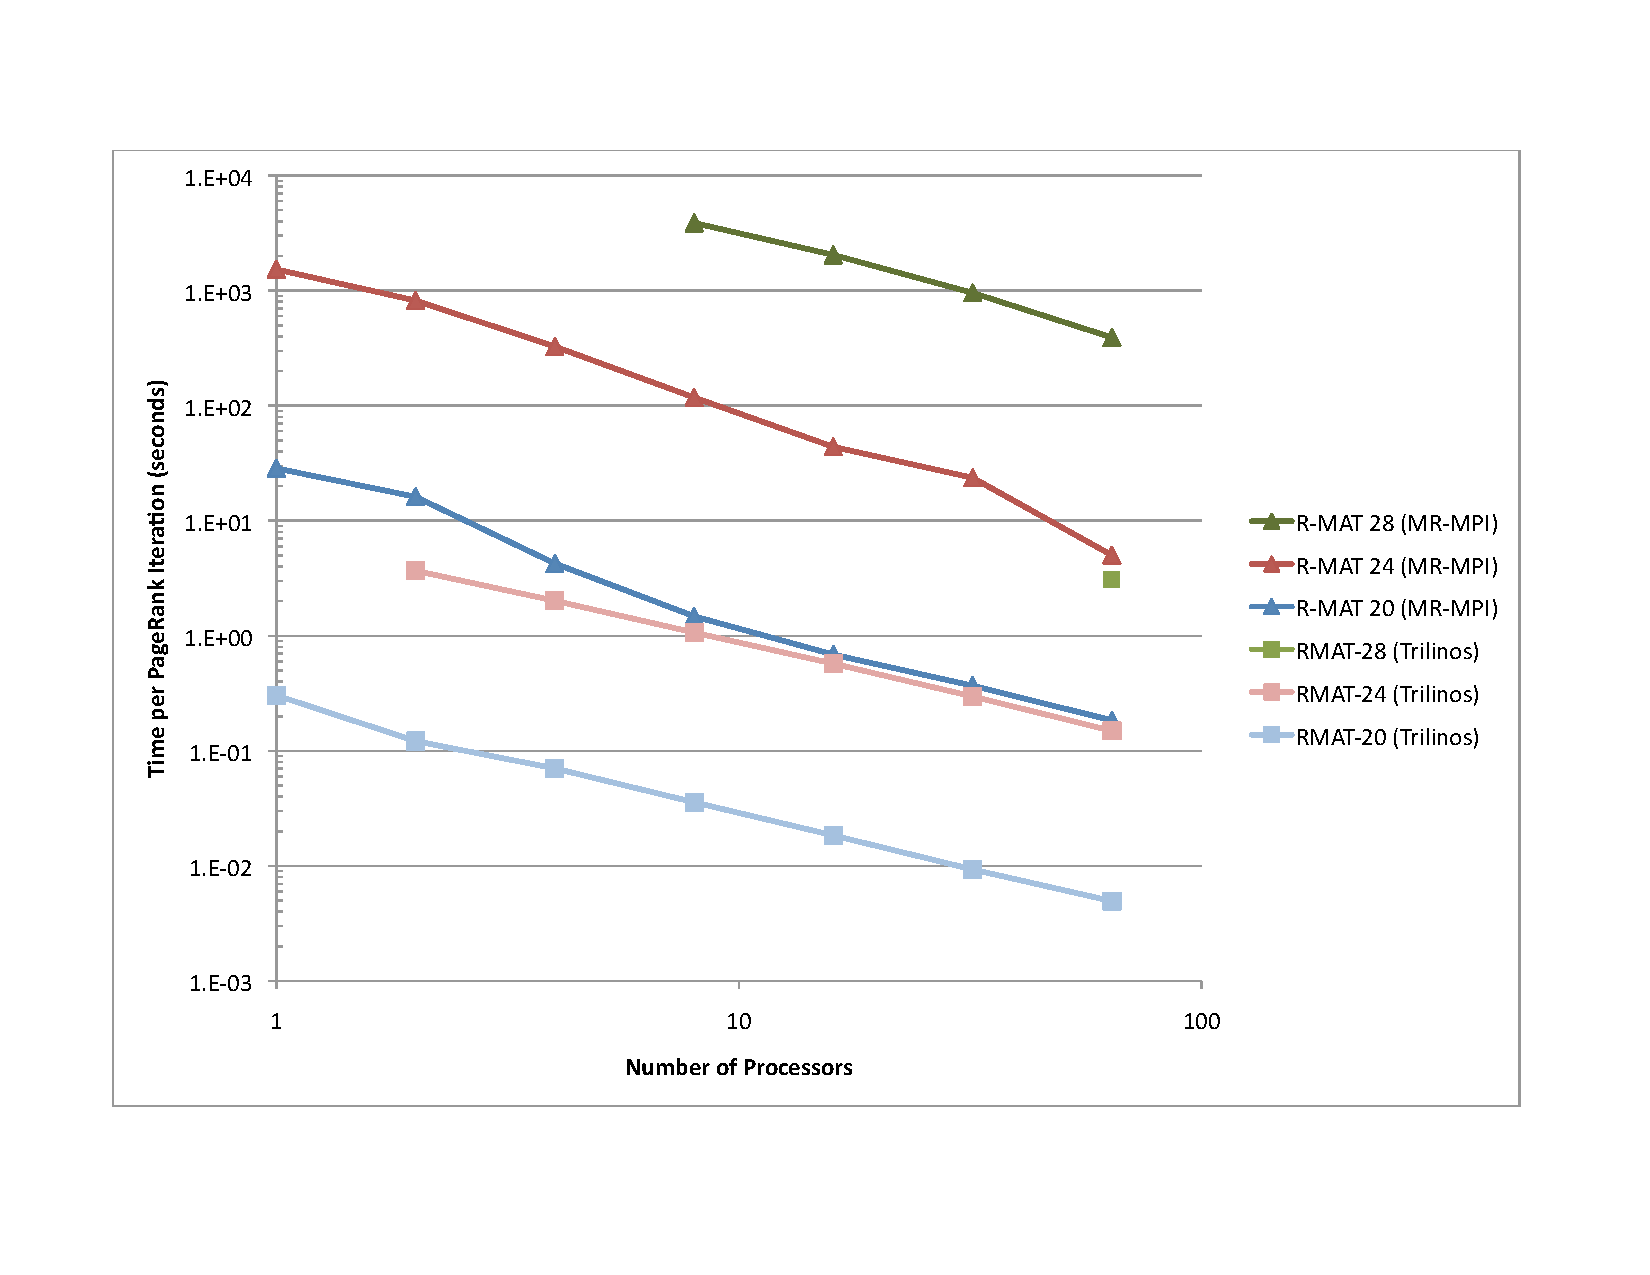
\includegraphics[width=\textwidth]{fig_pagerank.pdf}
\caption{Comparison of PageRank implementations using MapReduce,
Trilinos, and MTGL on R-MAT data sets.}
\label{fig:pr}
\end{figure}



\subsection{Triangle finding results}
Discuss triangle finding times.


\subsection{Maximally independent set results}
Discuss Luby maximally independent sets times.

\subsection{Single-source shortest path results}
Discuss SSSP times.

\subsection{Scalability to large numbers of processors}
Finally, we demonstrate the scalability of MR-MPI to large numbers of 
processors.  
The MR-MPI implementation was run on the Redstorm and Thunderbird
parallel computers
Because these systems do not have local disks for each processor, we selected 
a data set and page sizes that fit in their memory, so out-of-core operations
were not used.  For these experiments, we used an R-MAT data set with 
with $2^{25}$ vertices and $2^{28}$ edges, with parameters given in
Table~\ref{t:rmat}.  We ran both PageRank and Connected Components
algorithms.

\begin{table}
\begin{tabular}{|l|c|c|c|c|c|c|c|}
\hline
Data & R-MAT  & R-MAT  & R-MAT  & R-MAT  & \# of    & \# of & Maximum \\
Set  & a      & b      & c      & d      & vertices & edges & vertex degree\\
\hline
nice  & 0.45 & 0.15 & 0.15 & 0.25 & $2^{25}$ & $2^{28}$ & 1108 \\
nasty & 0.57 & 0.19 & 0.19 & 0.05 & $2^{25}$ & $2^{28}$ & 230,207\\
\hline
\end{tabular}
\caption{Characteristics of R-MAT input data for PageRank and Connected
Components scalability experiments.}
\label{t:rmat}
\end{table}

In Figure~\ref{fig:prbig}, we show the performance 
of the various PageRank
implementations on distributed memory and multi-threaded architectures.
The MR-MPI implementation demonstrated good scalability up to 1024 processors; 
however, it required an order-of-magnitude
more execution time than the matrix-based implementations on Redstorm.  
The distributed memory matrix-based
implementations are competitive with the multi-threaded implementation
in MTGL on the Cray XMT.

\begin{figure}[h!]
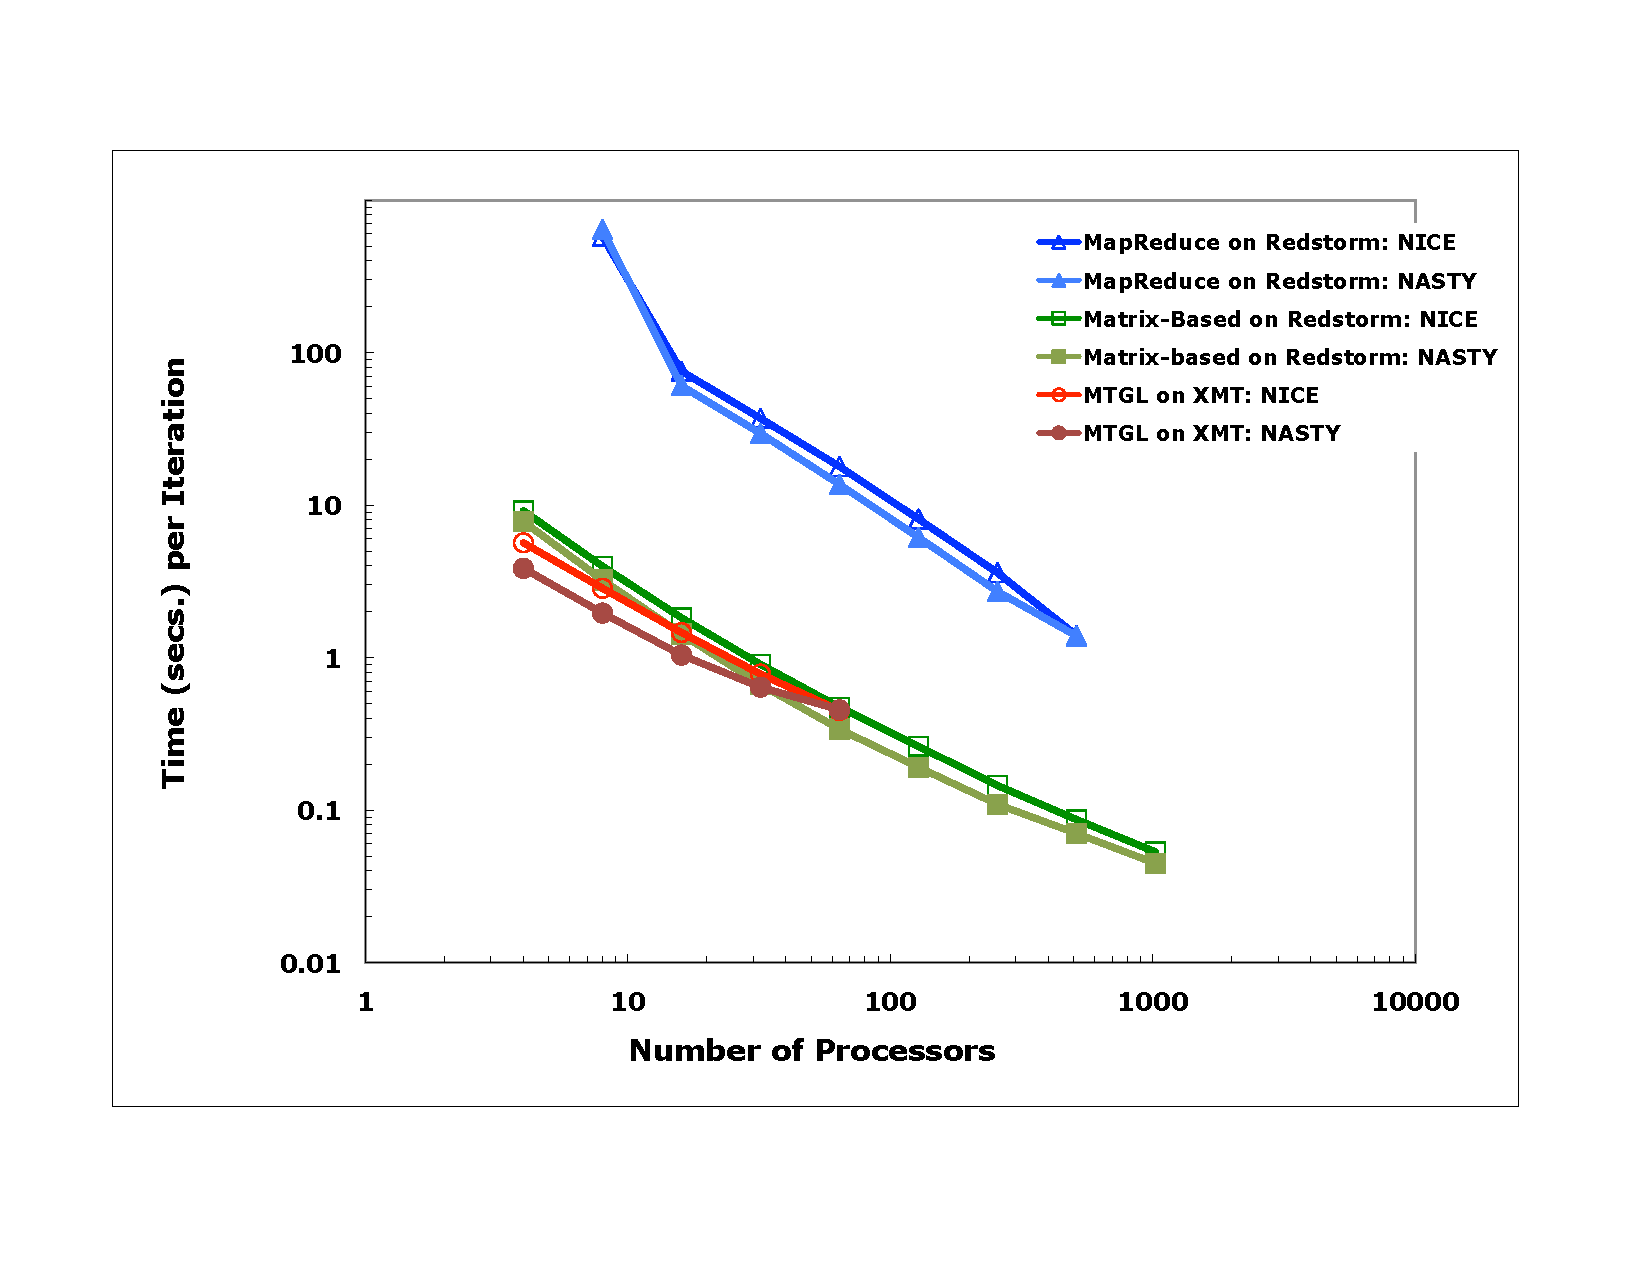
\includegraphics[width=\textwidth]{fig_pagerank_big.pdf}
\caption{Scalability comparison of PageRank implementations using MapReduce,
Trilinos, and MTGL on R-MAT data sets.}
\label{fig:prbig}
\end{figure}

Similar results were obtained for the Connected Components algorithm, as
we show in Figure~\ref{fig:ccbig}.  As with PageRank, the MR-MPI implementation
showed good scalability up to 1024 processors, but required significantly
more time than the Giant Connected Components algorithms using MTGL and
Trilinos.

\begin{figure}[h!]
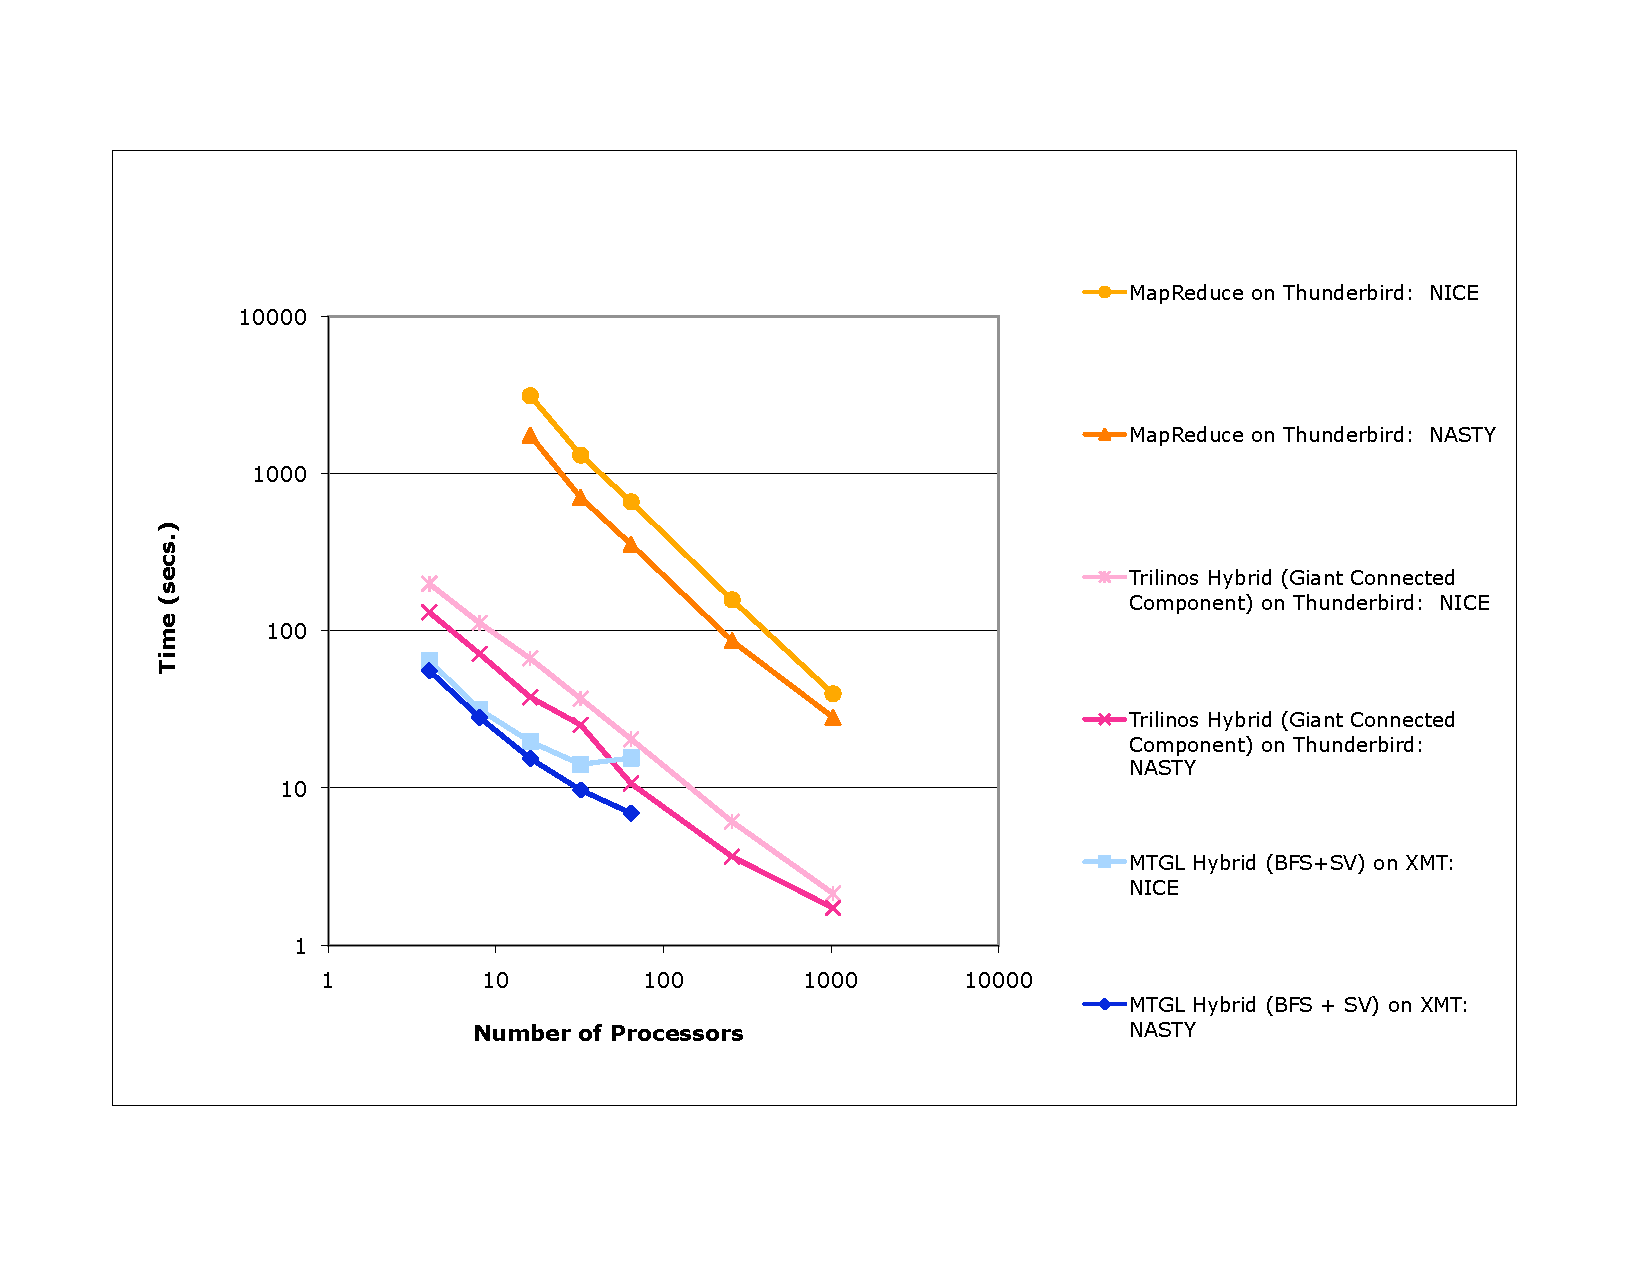
\includegraphics[width=\textwidth]{fig_cc_big.pdf}
\caption{Scalability comparison of Connected Components implementations using MapReduce,
Trilinos, and MTGL on R-MAT data sets.}
\label{fig:ccbig}
\end{figure}


\section{Lessons Learned}
\label{sec:lessons}

We conclude with several observations about performing MapReduce
operations on distributed-memory parallel machines via MPI.

MapReduce achieves parallelism through randomizing the distribution of
data across processors, which often intentionally ignores data
locality.  This translates into maximal data movement (during a
shuffle) with communication between all pairs of processors.  But the
benefit is often good load-balance, even for hard-to-balance irregular
data sets.  By contrast, more traditional distributed-memory parallel
algorithms, e.g. for matrix operations, or grid-based or
particle-based simulation codes, tend to work hard to localize data
and minimize communication.  To do this they typically require a lot
of application-specific logic and parallel communication coding, to
create and maintain a data decomposition, generate ghost versions of
nearby spatially-decomposed data, etc.

MapReduce algorithms can be hard to design, but are often relatively
easy to write and debug.  Thinking about a computational task from a
MapReduce perspective is different than traditional distributed-memory
parallel algorithm design.  For example, with an MPI mindset, it often
seems heretical to intentionally ignore data locality.  However,
writing small map() and reduce() functions is typically easy.  And
writing an algorithm that involves complex parallel operations,
without actually needing to write application-specific parallel code
to move data via MPI calls, is often a pleasant surprise.  Moreover,
if the MapReduce algorithm is initially coded so that it runs
correctly on one processor, it often works out-of-the-box on hundreds
or thousands of processors, without the need for additional debugging.

Performing MapReduce operations on a fixed allocation of processors on
a traditional MPI-based parallel machine is a somewhat different
conceptual model than that of cloud-computing MapReduces using (for
example) Hadoop.  In the former case, one can potentially control
which processor owns which data at various stages of an algorithm.
This is somewhat hidden from the user in a typical cloud-computing
model, where data simply exists somehere in the cloud, and Hadoop
ensures data moves where it needs to and is operated on by some
processor.  The cloud model is a nice data-centric abstraction which
allows for fault tolerance both to data loss (via redundant storage)
and to processor failure (via reassignment of work), neither of which
is typically possible on current MPI-based parallel machines.

However, since the MPI implementation of MapReduce, at least as
described in this paper, is processor-centric, one can sometimes
fruitfully exploit the possibility for processors to maintain
``state'' over the course of multiple map and reduce operations.  By
controlling where data resides for maps and reduces (e.g. via a
user-specified hash function), and by assuming that processor will
always be available, more efficient operations with less data movement
are sometimes possible.  The discussion of enhanced graph algorithms
in Section \ref{sec:graph} illustrated this.  To fully exploit this
idea for large data sets, mechanisms are needed for processors to
store, retrieve, and efficiently find needed datums on local disk
(e.g. static edges of a graph), so that archived state can be used
efficiently during subsequent map and reduce operations.

Finally, though this paper focuses on graph algorithms expressed as
MapReduce operations, there is nothing about the MR-MPI library itself
that is graph centric.  We hope the library can be generally useful on
large-scale monolithic or cloud-style parallel machines which support
MPI, for a variety of data-intense or compute-intense problems that
are amenable to solution using a MapReduce paradigm.

\section{Acknowledgments}
\label{sec:thanks}

The MR-MPI library is open-source software, which can be downloaded
from \url{http://www.sandia.gov/~sjplimp/mapreduce.html}.  It is
freely available under the terms of a BSD license.  Benchmark programs
which call the library to implement the algorithms of and which
produced the timing results of Section~\ref{sec:results} are included
in the distribution.

We thank the following individuals for their contributions to this
paper: Greg Bayer and Todd Plantenga (Sandia) for explaining Hadoop
concepts to us, and for the Hadoop implementations and timings of
Section~\ref{sec:results}; Jon Cohen (DoD) for fruitful discussions
about his MapReduce graph algorithms~\cite{Cohen09}; Brian Barrett
(Sandia) for the PBGL results of Section~\ref{sec:results}; Jon Berry
(Sandia) for the MTGL results of Section~\ref{sec:results}, and for
his overall support of this work and many useful discussions.

Sandia National Laboratories is a multi-program laboratory operated by
Sandia Corporation, a wholly owned subsidiary of Lockheed Martin
company, for the U.S. Department of Energy's National Nuclear Security
Administration under contract DE-AC04-94AL85000.


\bibliographystyle{abbrv}
\bibliography{paper}

\end{document}
